\begin{frame}
  \frametitle{Outline}
  \tableofcontents
\end{frame}

\begin{section}{Introduction}
  \begin{frame}
    \frametitle{Introduction}
  \end{frame}

  \begin{frame}
    \frametitle{Field Theories in Nature}
    \begin{itemize}
    \item The Standard Model of elementary particles
    \item The theory of gravitation
    \item Hydrodynamics
    \item Neuron activity in the brain
    \end{itemize}
  \end{frame}

  \begin{frame}
    \frametitle{Field theory reminds}
    A field theory is defined by its Lagrangian density, or action:
    \begin{equation*}
      S = \int\mathrm d^4 x \mathcal L(x^\mu,\phi, \partial_\mu\phi).
    \end{equation*}
    The first order of variation of the action must vanish around the
    classical field configuration:
    \begin{equation*}
      \delta S = \int\mathrm d^4 x\delta\mathcal L(x^\mu,\phi, \partial_\mu\phi),
    \end{equation*}
    leading to the field equations:
    \begin{equation*}
      \frac{\partial \mathcal L}{\partial \phi}-\partial_\mu\frac{\partial\mathcal L}{\partial\partial_\mu\phi}=0.
    \end{equation*}
    \end{frame}

    \begin{frame}
      \frametitle{A particular field configuration: Soliton}
      A soliton is a solution of the field equation which:
      \begin{itemize}
      \item is time independant
      \item has a finite energy
      \end{itemize}
      Many modern particle theories exibit such solutions on the
      classical level.

      They are very popular in cosmology:
      \begin{itemize}
      \item Cosmic strings, domain walls, and attempts to localize gravity, wrap dimensions
      \item Magnetic monopoles as WIMPs
      \item Monopoles are a feature of many GUTs
      \end{itemize}
    \end{frame}

    \begin{frame}
      \frametitle{A particular field configuration: Instanton}
      An instanton is a solution of the field equations which is
      \begin{itemize}
      \item in euclidian time,
      \item localised in time and space.
      \end{itemize}
      Again, instanton is common in many nowadays theories.
    \end{frame}

\end{section}

\begin{section}{Mathematical Framework}
  \begin{frame}
    \frametitle{Mathematical Framework}
  \end{frame}

  \begin{frame}
    \frametitle{The problem of analytic continuation}
    The situation
    arise when we have a field configuration in Minkowski time we
    want to evaluate in Euclidian time:

    \begin{equation}
      r=\sqrt{x^2+\tau^2}\xrightarrow{\tau\to -it}\sqrt{x^2-t^2}.
    \end{equation}
    If $t>x$:
    \begin{equation*}
      r = \pm i \sqrt{|t^2-x^2|} = \pm i s.
    \end{equation*}
  \end{frame}

  \begin{frame}
    \frametitle{The problem of analytic continuation}
    Let $\vec f(r)$ be a function defined by:
    \begin{equation*}
      \vec f'(x) = \vec F(x, \vec f(x)).
    \end{equation*}
    The analytic continuation of $f(r)$, noted $\tilde f(z)$ is
    obtained by extending the derivative to the complex part:
    \begin{align*}
      &f'(x)\to \frac{\partial f}{\partial z}\equiv \partial_x f_{\mathrm R}(x+iy)+i\partial_x f_{\mathrm I}(x+iy),\\
      &\Rightarrow \partial_x f_{\mathrm R}(z)+i\partial_x f_{\mathrm I}(z) = F_{\mathrm R}(z,\tilde f(z))+F_{\mathrm I}(z,\tilde f(z)).
    \end{align*}
  \end{frame}
  \begin{frame}
    \frametitle{Cauchy-Riemann equations}
    The Cauchy-Riemann equations allow us to write the system in terms of the derivatives w.r.t the complex coordinate:
    \begin{align*}
      &\left\{\begin{aligned}
      &\partial_x f_{\mathrm R} = \partial_y f_{\mathrm I},\\
      &\partial_x f_{\mathrm I} = -\partial_y f_{\mathrm R},
      \end{aligned}\right.
    \end{align*}
    which lead to the Cauchy problem:
    \begin{align*}
      \Rightarrow&\left\{\begin{aligned}
      &\partial_y f_{\mathrm I} = F_{\mathrm R}(z,\tilde f(z)),\\
      &\partial_y f_{\mathrm R} = -F_{\mathrm I}(z,\tilde f(z)).
      \end{aligned}\right.
    \end{align*}
  \end{frame}
  \begin{frame}
    \frametitle{Choice of coordinate system}
    This is not enough in the following situation:
    %% Creator: Inkscape inkscape 0.48.2, www.inkscape.org
%% PDF/EPS/PS + LaTeX output extension by Johan Engelen, 2010
%% Accompanies image file 'coordeffect.pdf' (pdf, eps, ps)
%%
%% To include the image in your LaTeX document, write
%%   \input{<filename>.pdf_tex}
%%  instead of
%%   \includegraphics{<filename>.pdf}
%% To scale the image, write
%%   \def\svgwidth{<desired width>}
%%   \input{<filename>.pdf_tex}
%%  instead of
%%   \includegraphics[width=<desired width>]{<filename>.pdf}
%%
%% Images with a different path to the parent latex file can
%% be accessed with the `import' package (which may need to be
%% installed) using
%%   \usepackage{import}
%% in the preamble, and then including the image with
%%   \import{<path to file>}{<filename>.pdf_tex}
%% Alternatively, one can specify
%%   \graphicspath{{<path to file>/}}
%% 
%% For more information, please see info/svg-inkscape on CTAN:
%%   http://tug.ctan.org/tex-archive/info/svg-inkscape
%%
\begingroup%
  \makeatletter%
  \providecommand\color[2][]{%
    \errmessage{(Inkscape) Color is used for the text in Inkscape, but the package 'color.sty' is not loaded}%
    \renewcommand\color[2][]{}%
  }%
  \providecommand\transparent[1]{%
    \errmessage{(Inkscape) Transparency is used (non-zero) for the text in Inkscape, but the package 'transparent.sty' is not loaded}%
    \renewcommand\transparent[1]{}%
  }%
  \providecommand\rotatebox[2]{#2}%
  \ifx\svgwidth\undefined%
    \setlength{\unitlength}{311.81101074bp}%
    \ifx\svgscale\undefined%
      \relax%
    \else%
      \setlength{\unitlength}{\unitlength * \real{\svgscale}}%
    \fi%
  \else%
    \setlength{\unitlength}{\svgwidth}%
  \fi%
  \global\let\svgwidth\undefined%
  \global\let\svgscale\undefined%
  \makeatother%
  \begin{picture}(1,0.40909093)%
    \put(0,0){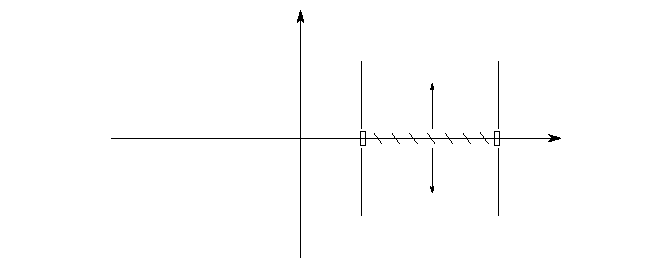
\includegraphics[width=\unitlength]{coordeffect.pdf}}%
    \put(0.81001449,0.15036999){\color[rgb]{0,0,0}\makebox(0,0)[lb]{\smash{$\Re(z)$}}}%
    \put(0.47647914,0.36377714){\color[rgb]{0,0,0}\makebox(0,0)[lb]{\smash{$\Im(z)$}}}%
  \end{picture}%
\endgroup%

    but can be addressed with a change of coordinate.
  \end{frame}
  \begin{frame}
    \frametitle{Change to polar coordinate}
    Define the new polar coordinates:
    \begin{align*}
      \left\{\begin{aligned}
      &x = r\cos\theta, \\
      &y = r\sin\theta.
      \end{aligned}\right.
    \end{align*}
    Using the Cauchy-Riemann equations, we can rewrite the previous
    Cauchy problem for the $\theta$ variable:
    \begin{align*}
      \begin{bmatrix}
      -\partial_\theta f_{\mathrm R}(r,\theta)\\
      \partial_\theta f_{\mathrm I}(r,\theta)
      \end{bmatrix}
      = r
      \begin{bmatrix}
        \cos\theta & \sin\theta\\
        -\sin\theta & \cos\theta\\
      \end{bmatrix}
      \begin{bmatrix}
        F_{\mathrm I}(z,\tilde f(z))\\
        F_{\mathrm R}(z,\tilde f(z))
      \end{bmatrix}.
    \end{align*}
  \end{frame}

\end{section}

\begin{section}{First tests}
  \begin{frame}
    \frametitle{First Tests}
    We now want to test the framework on a set of known functions:
    \begin{itemize}
    \item The square root
    \item The natural logarithm
    \item An instanton of the quantum pendulum equation
    \end{itemize}
  \end{frame}

  \begin{frame}
    \frametitle{The square root}
    \begin{enumerate}
    \item The square root is defined by the differential equation:
      \begin{align*}
        f(x) = \sqrt{x} \Rightarrow f'(x) = \frac{1}{2}\frac{1}{\sqrt{x}} = \frac{1}{2f(x)},
      \end{align*}
      \item which leads to the Cauchy problem:
        \begin{align*}
          \left\{
          \begin{aligned}
            &\partial_yf_I(z) = \frac{f_R(z)}{2(f_R^2(z)+f_I^2(z))}\\
            &-\partial_yf_R(z) = -\frac{f_I(z)}{2(f_R^2(z)+f_I^2(z))}
          \end{aligned}
          \qquad
          \right|
          \qquad
          \begin{aligned}
            &f_{\mathrm R}(x+i0) = \sqrt{x}\\
            &f_{\mathrm I}(x+i0) = 0
          \end{aligned}
        \end{align*}
    \end{enumerate}
  \end{frame}
  \begin{frame}
    \frametitle{Numerical analytic continuation of the Square Root}
    % GNUPLOT: LaTeX picture with Postscript
\begingroup
\scriptsize
  \makeatletter
  \providecommand\color[2][]{%
    \GenericError{(gnuplot) \space\space\space\@spaces}{%
      Package color not loaded in conjunction with
      terminal option `colourtext'%
    }{See the gnuplot documentation for explanation.%
    }{Either use 'blacktext' in gnuplot or load the package
      color.sty in LaTeX.}%
    \renewcommand\color[2][]{}%
  }%
  \providecommand\includegraphics[2][]{%
    \GenericError{(gnuplot) \space\space\space\@spaces}{%
      Package graphicx or graphics not loaded%
    }{See the gnuplot documentation for explanation.%
    }{The gnuplot epslatex terminal needs graphicx.sty or graphics.sty.}%
    \renewcommand\includegraphics[2][]{}%
  }%
  \providecommand\rotatebox[2]{#2}%
  \@ifundefined{ifGPcolor}{%
    \newif\ifGPcolor
    \GPcolortrue
  }{}%
  \@ifundefined{ifGPblacktext}{%
    \newif\ifGPblacktext
    \GPblacktexttrue
  }{}%
  % define a \g@addto@macro without @ in the name:
  \let\gplgaddtomacro\g@addto@macro
  % define empty templates for all commands taking text:
  \gdef\gplbacktext{}%
  \gdef\gplfronttext{}%
  \makeatother
  \ifGPblacktext
    % no textcolor at all
    \def\colorrgb#1{}%
    \def\colorgray#1{}%
  \else
    % gray or color?
    \ifGPcolor
      \def\colorrgb#1{\color[rgb]{#1}}%
      \def\colorgray#1{\color[gray]{#1}}%
      \expandafter\def\csname LTw\endcsname{\color{white}}%
      \expandafter\def\csname LTb\endcsname{\color{black}}%
      \expandafter\def\csname LTa\endcsname{\color{black}}%
      \expandafter\def\csname LT0\endcsname{\color[rgb]{1,0,0}}%
      \expandafter\def\csname LT1\endcsname{\color[rgb]{0,1,0}}%
      \expandafter\def\csname LT2\endcsname{\color[rgb]{0,0,1}}%
      \expandafter\def\csname LT3\endcsname{\color[rgb]{1,0,1}}%
      \expandafter\def\csname LT4\endcsname{\color[rgb]{0,1,1}}%
      \expandafter\def\csname LT5\endcsname{\color[rgb]{1,1,0}}%
      \expandafter\def\csname LT6\endcsname{\color[rgb]{0,0,0}}%
      \expandafter\def\csname LT7\endcsname{\color[rgb]{1,0.3,0}}%
      \expandafter\def\csname LT8\endcsname{\color[rgb]{0.5,0.5,0.5}}%
    \else
      % gray
      \def\colorrgb#1{\color{black}}%
      \def\colorgray#1{\color[gray]{#1}}%
      \expandafter\def\csname LTw\endcsname{\color{white}}%
      \expandafter\def\csname LTb\endcsname{\color{black}}%
      \expandafter\def\csname LTa\endcsname{\color{black}}%
      \expandafter\def\csname LT0\endcsname{\color{black}}%
      \expandafter\def\csname LT1\endcsname{\color{black}}%
      \expandafter\def\csname LT2\endcsname{\color{black}}%
      \expandafter\def\csname LT3\endcsname{\color{black}}%
      \expandafter\def\csname LT4\endcsname{\color{black}}%
      \expandafter\def\csname LT5\endcsname{\color{black}}%
      \expandafter\def\csname LT6\endcsname{\color{black}}%
      \expandafter\def\csname LT7\endcsname{\color{black}}%
      \expandafter\def\csname LT8\endcsname{\color{black}}%
    \fi
  \fi
  \setlength{\unitlength}{0.0500bp}%
  \begin{picture}(2834.00,2834.00)%
    \gplgaddtomacro\gplbacktext{%
      \csname LTb\endcsname%
      \put(473,998){\makebox(0,0){\strut{}-1}}%
      \put(873,745){\makebox(0,0){\strut{} 0}}%
      \put(1273,491){\makebox(0,0){\strut{} 1}}%
      \put(1550,503){\makebox(0,0){\strut{}-1}}%
      \put(1950,756){\makebox(0,0){\strut{} 0}}%
      \put(2350,1009){\makebox(0,0){\strut{} 1}}%
      \put(411,1420){\makebox(0,0)[r]{\strut{}-1}}%
      \put(411,1658){\makebox(0,0)[r]{\strut{} 0}}%
      \put(411,1897){\makebox(0,0)[r]{\strut{} 1}}%
      \put(54,1358){\rotatebox{90}{\makebox(0,0){\strut{}$\Re\sqrt{x+iy}$}}}%
    }%
    \gplgaddtomacro\gplfronttext{%
      \csname LTb\endcsname%
      \put(626,496){\makebox(0,0){\strut{}$x$}}%
      \put(2209,496){\makebox(0,0){\strut{}$y$}}%
      \put(54,1358){\rotatebox{90}{\makebox(0,0){\strut{}$\Re\sqrt{x+iy}$}}}%
      \put(2517,1395){\makebox(0,0)[l]{\strut{}-1}}%
      \put(2517,1722){\makebox(0,0)[l]{\strut{} 0}}%
      \put(2517,2048){\makebox(0,0)[l]{\strut{} 1}}%
    }%
    \gplbacktext
    \put(0,0){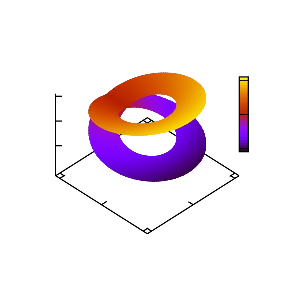
\includegraphics{sqrt_riemann_real}}%
    \gplfronttext
  \end{picture}%
\endgroup

    % GNUPLOT: LaTeX picture with Postscript
\begingroup
\scriptsize
  \makeatletter
  \providecommand\color[2][]{%
    \GenericError{(gnuplot) \space\space\space\@spaces}{%
      Package color not loaded in conjunction with
      terminal option `colourtext'%
    }{See the gnuplot documentation for explanation.%
    }{Either use 'blacktext' in gnuplot or load the package
      color.sty in LaTeX.}%
    \renewcommand\color[2][]{}%
  }%
  \providecommand\includegraphics[2][]{%
    \GenericError{(gnuplot) \space\space\space\@spaces}{%
      Package graphicx or graphics not loaded%
    }{See the gnuplot documentation for explanation.%
    }{The gnuplot epslatex terminal needs graphicx.sty or graphics.sty.}%
    \renewcommand\includegraphics[2][]{}%
  }%
  \providecommand\rotatebox[2]{#2}%
  \@ifundefined{ifGPcolor}{%
    \newif\ifGPcolor
    \GPcolortrue
  }{}%
  \@ifundefined{ifGPblacktext}{%
    \newif\ifGPblacktext
    \GPblacktexttrue
  }{}%
  % define a \g@addto@macro without @ in the name:
  \let\gplgaddtomacro\g@addto@macro
  % define empty templates for all commands taking text:
  \gdef\gplbacktext{}%
  \gdef\gplfronttext{}%
  \makeatother
  \ifGPblacktext
    % no textcolor at all
    \def\colorrgb#1{}%
    \def\colorgray#1{}%
  \else
    % gray or color?
    \ifGPcolor
      \def\colorrgb#1{\color[rgb]{#1}}%
      \def\colorgray#1{\color[gray]{#1}}%
      \expandafter\def\csname LTw\endcsname{\color{white}}%
      \expandafter\def\csname LTb\endcsname{\color{black}}%
      \expandafter\def\csname LTa\endcsname{\color{black}}%
      \expandafter\def\csname LT0\endcsname{\color[rgb]{1,0,0}}%
      \expandafter\def\csname LT1\endcsname{\color[rgb]{0,1,0}}%
      \expandafter\def\csname LT2\endcsname{\color[rgb]{0,0,1}}%
      \expandafter\def\csname LT3\endcsname{\color[rgb]{1,0,1}}%
      \expandafter\def\csname LT4\endcsname{\color[rgb]{0,1,1}}%
      \expandafter\def\csname LT5\endcsname{\color[rgb]{1,1,0}}%
      \expandafter\def\csname LT6\endcsname{\color[rgb]{0,0,0}}%
      \expandafter\def\csname LT7\endcsname{\color[rgb]{1,0.3,0}}%
      \expandafter\def\csname LT8\endcsname{\color[rgb]{0.5,0.5,0.5}}%
    \else
      % gray
      \def\colorrgb#1{\color{black}}%
      \def\colorgray#1{\color[gray]{#1}}%
      \expandafter\def\csname LTw\endcsname{\color{white}}%
      \expandafter\def\csname LTb\endcsname{\color{black}}%
      \expandafter\def\csname LTa\endcsname{\color{black}}%
      \expandafter\def\csname LT0\endcsname{\color{black}}%
      \expandafter\def\csname LT1\endcsname{\color{black}}%
      \expandafter\def\csname LT2\endcsname{\color{black}}%
      \expandafter\def\csname LT3\endcsname{\color{black}}%
      \expandafter\def\csname LT4\endcsname{\color{black}}%
      \expandafter\def\csname LT5\endcsname{\color{black}}%
      \expandafter\def\csname LT6\endcsname{\color{black}}%
      \expandafter\def\csname LT7\endcsname{\color{black}}%
      \expandafter\def\csname LT8\endcsname{\color{black}}%
    \fi
  \fi
  \setlength{\unitlength}{0.0500bp}%
  \begin{picture}(2834.00,2834.00)%
    \gplgaddtomacro\gplbacktext{%
      \csname LTb\endcsname%
      \put(473,998){\makebox(0,0){\strut{}-1}}%
      \put(873,745){\makebox(0,0){\strut{} 0}}%
      \put(1273,491){\makebox(0,0){\strut{} 1}}%
      \put(1550,503){\makebox(0,0){\strut{}-1}}%
      \put(1950,756){\makebox(0,0){\strut{} 0}}%
      \put(2350,1009){\makebox(0,0){\strut{} 1}}%
      \put(411,1420){\makebox(0,0)[r]{\strut{}-1}}%
      \put(411,1658){\makebox(0,0)[r]{\strut{} 0}}%
      \put(411,1897){\makebox(0,0)[r]{\strut{} 1}}%
      \put(54,1358){\rotatebox{90}{\makebox(0,0){\strut{}$\Im\sqrt{x+iy}$}}}%
    }%
    \gplgaddtomacro\gplfronttext{%
      \csname LTb\endcsname%
      \put(626,496){\makebox(0,0){\strut{}$x$}}%
      \put(2209,496){\makebox(0,0){\strut{}$y$}}%
      \put(54,1358){\rotatebox{90}{\makebox(0,0){\strut{}$\Im\sqrt{x+iy}$}}}%
      \put(2517,1395){\makebox(0,0)[l]{\strut{}-1}}%
      \put(2517,1722){\makebox(0,0)[l]{\strut{} 0}}%
      \put(2517,2048){\makebox(0,0)[l]{\strut{} 1}}%
    }%
    \gplbacktext
    \put(0,0){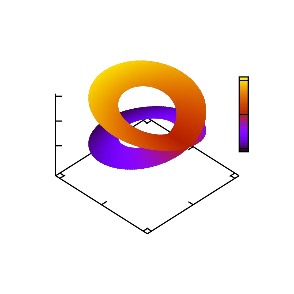
\includegraphics{sqrt_riemann_imag}}%
    \gplfronttext
  \end{picture}%
\endgroup

  \end{frame}

  \begin{frame}
    \frametitle{The Natural Logarithm}
    \begin{enumerate}
    \item The natural logarithm is defined by the differential equation:
      \begin{align*}
        f(x) = \log(x) \Rightarrow f'(x) = \frac{1}{x} = \exp(-f(x)),
      \end{align*}
      \item which leads to the Cauchy problem:
        \begin{align*}
          \left\{
          \begin{aligned}
            &\partial_yf_I(z) = \exp(-f_R(z))\cos(f_I)\\
            &-\partial_yf_R(z) = -\exp(-f_R(z))\sin(f_I)
          \end{aligned}
          \qquad
          \right|
          \qquad
          \begin{aligned}
            &f_{\mathrm R}(x+i0) = \log(x)\\
            &f_{\mathrm I}(x+i0) = 0
          \end{aligned}
        \end{align*}
    \end{enumerate}
  \end{frame}
  \begin{frame}
    \frametitle{Numerical analytic continuation of the Logarithm}
    % GNUPLOT: LaTeX picture with Postscript
\begingroup
\scriptsize
  \makeatletter
  \providecommand\color[2][]{%
    \GenericError{(gnuplot) \space\space\space\@spaces}{%
      Package color not loaded in conjunction with
      terminal option `colourtext'%
    }{See the gnuplot documentation for explanation.%
    }{Either use 'blacktext' in gnuplot or load the package
      color.sty in LaTeX.}%
    \renewcommand\color[2][]{}%
  }%
  \providecommand\includegraphics[2][]{%
    \GenericError{(gnuplot) \space\space\space\@spaces}{%
      Package graphicx or graphics not loaded%
    }{See the gnuplot documentation for explanation.%
    }{The gnuplot epslatex terminal needs graphicx.sty or graphics.sty.}%
    \renewcommand\includegraphics[2][]{}%
  }%
  \providecommand\rotatebox[2]{#2}%
  \@ifundefined{ifGPcolor}{%
    \newif\ifGPcolor
    \GPcolortrue
  }{}%
  \@ifundefined{ifGPblacktext}{%
    \newif\ifGPblacktext
    \GPblacktexttrue
  }{}%
  % define a \g@addto@macro without @ in the name:
  \let\gplgaddtomacro\g@addto@macro
  % define empty templates for all commands taking text:
  \gdef\gplbacktext{}%
  \gdef\gplfronttext{}%
  \makeatother
  \ifGPblacktext
    % no textcolor at all
    \def\colorrgb#1{}%
    \def\colorgray#1{}%
  \else
    % gray or color?
    \ifGPcolor
      \def\colorrgb#1{\color[rgb]{#1}}%
      \def\colorgray#1{\color[gray]{#1}}%
      \expandafter\def\csname LTw\endcsname{\color{white}}%
      \expandafter\def\csname LTb\endcsname{\color{black}}%
      \expandafter\def\csname LTa\endcsname{\color{black}}%
      \expandafter\def\csname LT0\endcsname{\color[rgb]{1,0,0}}%
      \expandafter\def\csname LT1\endcsname{\color[rgb]{0,1,0}}%
      \expandafter\def\csname LT2\endcsname{\color[rgb]{0,0,1}}%
      \expandafter\def\csname LT3\endcsname{\color[rgb]{1,0,1}}%
      \expandafter\def\csname LT4\endcsname{\color[rgb]{0,1,1}}%
      \expandafter\def\csname LT5\endcsname{\color[rgb]{1,1,0}}%
      \expandafter\def\csname LT6\endcsname{\color[rgb]{0,0,0}}%
      \expandafter\def\csname LT7\endcsname{\color[rgb]{1,0.3,0}}%
      \expandafter\def\csname LT8\endcsname{\color[rgb]{0.5,0.5,0.5}}%
    \else
      % gray
      \def\colorrgb#1{\color{black}}%
      \def\colorgray#1{\color[gray]{#1}}%
      \expandafter\def\csname LTw\endcsname{\color{white}}%
      \expandafter\def\csname LTb\endcsname{\color{black}}%
      \expandafter\def\csname LTa\endcsname{\color{black}}%
      \expandafter\def\csname LT0\endcsname{\color{black}}%
      \expandafter\def\csname LT1\endcsname{\color{black}}%
      \expandafter\def\csname LT2\endcsname{\color{black}}%
      \expandafter\def\csname LT3\endcsname{\color{black}}%
      \expandafter\def\csname LT4\endcsname{\color{black}}%
      \expandafter\def\csname LT5\endcsname{\color{black}}%
      \expandafter\def\csname LT6\endcsname{\color{black}}%
      \expandafter\def\csname LT7\endcsname{\color{black}}%
      \expandafter\def\csname LT8\endcsname{\color{black}}%
    \fi
  \fi
  \setlength{\unitlength}{0.0500bp}%
  \begin{picture}(2834.00,2834.00)%
    \gplgaddtomacro\gplbacktext{%
      \csname LTb\endcsname%
      \put(473,938){\makebox(0,0){\strut{}-1}}%
      \put(873,816){\makebox(0,0){\strut{} 0}}%
      \put(1273,693){\makebox(0,0){\strut{} 1}}%
      \put(1550,699){\makebox(0,0){\strut{}-1}}%
      \put(1950,821){\makebox(0,0){\strut{} 0}}%
      \put(2350,944){\makebox(0,0){\strut{} 1}}%
      \put(411,1385){\makebox(0,0)[r]{\strut{}-1}}%
      \put(411,1701){\makebox(0,0)[r]{\strut{} 0}}%
      \put(411,2019){\makebox(0,0)[r]{\strut{} 1}}%
      \put(54,1330){\rotatebox{90}{\makebox(0,0){\strut{}$\Re\log(x+iy)$}}}%
    }%
    \gplgaddtomacro\gplfronttext{%
      \csname LTb\endcsname%
      \put(626,582){\makebox(0,0){\strut{}$x$}}%
      \put(2209,582){\makebox(0,0){\strut{}$y$}}%
      \put(54,1330){\rotatebox{90}{\makebox(0,0){\strut{}$\Re\log(x+iy)$}}}%
      \put(2517,1363){\makebox(0,0)[l]{\strut{}-1}}%
      \put(2517,1722){\makebox(0,0)[l]{\strut{} 0}}%
      \put(2517,2081){\makebox(0,0)[l]{\strut{} 1}}%
    }%
    \gplbacktext
    \put(0,0){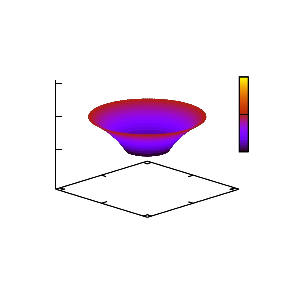
\includegraphics{log_riemann_real}}%
    \gplfronttext
  \end{picture}%
\endgroup

    % GNUPLOT: LaTeX picture with Postscript
\begingroup
\scriptsize
  \makeatletter
  \providecommand\color[2][]{%
    \GenericError{(gnuplot) \space\space\space\@spaces}{%
      Package color not loaded in conjunction with
      terminal option `colourtext'%
    }{See the gnuplot documentation for explanation.%
    }{Either use 'blacktext' in gnuplot or load the package
      color.sty in LaTeX.}%
    \renewcommand\color[2][]{}%
  }%
  \providecommand\includegraphics[2][]{%
    \GenericError{(gnuplot) \space\space\space\@spaces}{%
      Package graphicx or graphics not loaded%
    }{See the gnuplot documentation for explanation.%
    }{The gnuplot epslatex terminal needs graphicx.sty or graphics.sty.}%
    \renewcommand\includegraphics[2][]{}%
  }%
  \providecommand\rotatebox[2]{#2}%
  \@ifundefined{ifGPcolor}{%
    \newif\ifGPcolor
    \GPcolortrue
  }{}%
  \@ifundefined{ifGPblacktext}{%
    \newif\ifGPblacktext
    \GPblacktexttrue
  }{}%
  % define a \g@addto@macro without @ in the name:
  \let\gplgaddtomacro\g@addto@macro
  % define empty templates for all commands taking text:
  \gdef\gplbacktext{}%
  \gdef\gplfronttext{}%
  \makeatother
  \ifGPblacktext
    % no textcolor at all
    \def\colorrgb#1{}%
    \def\colorgray#1{}%
  \else
    % gray or color?
    \ifGPcolor
      \def\colorrgb#1{\color[rgb]{#1}}%
      \def\colorgray#1{\color[gray]{#1}}%
      \expandafter\def\csname LTw\endcsname{\color{white}}%
      \expandafter\def\csname LTb\endcsname{\color{black}}%
      \expandafter\def\csname LTa\endcsname{\color{black}}%
      \expandafter\def\csname LT0\endcsname{\color[rgb]{1,0,0}}%
      \expandafter\def\csname LT1\endcsname{\color[rgb]{0,1,0}}%
      \expandafter\def\csname LT2\endcsname{\color[rgb]{0,0,1}}%
      \expandafter\def\csname LT3\endcsname{\color[rgb]{1,0,1}}%
      \expandafter\def\csname LT4\endcsname{\color[rgb]{0,1,1}}%
      \expandafter\def\csname LT5\endcsname{\color[rgb]{1,1,0}}%
      \expandafter\def\csname LT6\endcsname{\color[rgb]{0,0,0}}%
      \expandafter\def\csname LT7\endcsname{\color[rgb]{1,0.3,0}}%
      \expandafter\def\csname LT8\endcsname{\color[rgb]{0.5,0.5,0.5}}%
    \else
      % gray
      \def\colorrgb#1{\color{black}}%
      \def\colorgray#1{\color[gray]{#1}}%
      \expandafter\def\csname LTw\endcsname{\color{white}}%
      \expandafter\def\csname LTb\endcsname{\color{black}}%
      \expandafter\def\csname LTa\endcsname{\color{black}}%
      \expandafter\def\csname LT0\endcsname{\color{black}}%
      \expandafter\def\csname LT1\endcsname{\color{black}}%
      \expandafter\def\csname LT2\endcsname{\color{black}}%
      \expandafter\def\csname LT3\endcsname{\color{black}}%
      \expandafter\def\csname LT4\endcsname{\color{black}}%
      \expandafter\def\csname LT5\endcsname{\color{black}}%
      \expandafter\def\csname LT6\endcsname{\color{black}}%
      \expandafter\def\csname LT7\endcsname{\color{black}}%
      \expandafter\def\csname LT8\endcsname{\color{black}}%
    \fi
  \fi
  \setlength{\unitlength}{0.0500bp}%
  \begin{picture}(2834.00,2834.00)%
    \gplgaddtomacro\gplbacktext{%
      \csname LTb\endcsname%
      \put(433,950){\makebox(0,0){\strut{}-1}}%
      \put(873,816){\makebox(0,0){\strut{} 0}}%
      \put(1313,681){\makebox(0,0){\strut{} 1}}%
      \put(1510,686){\makebox(0,0){\strut{}-1}}%
      \put(1950,821){\makebox(0,0){\strut{} 0}}%
      \put(2390,956){\makebox(0,0){\strut{} 1}}%
      \put(411,1357){\makebox(0,0)[r]{\strut{} 0}}%
      \put(411,1586){\makebox(0,0)[r]{\strut{} 5}}%
      \put(411,1816){\makebox(0,0)[r]{\strut{} 10}}%
      \put(411,2046){\makebox(0,0)[r]{\strut{} 15}}%
      \put(54,1330){\rotatebox{90}{\makebox(0,0){\strut{}$\Im\log(x+iy)$}}}%
    }%
    \gplgaddtomacro\gplfronttext{%
      \csname LTb\endcsname%
      \put(626,582){\makebox(0,0){\strut{}$x$}}%
      \put(2209,582){\makebox(0,0){\strut{}$y$}}%
      \put(54,1330){\rotatebox{90}{\makebox(0,0){\strut{}$\Im\log(x+iy)$}}}%
      \put(2517,1363){\makebox(0,0)[l]{\strut{} 0}}%
      \put(2517,1722){\makebox(0,0)[l]{\strut{} 7.5}}%
      \put(2517,2081){\makebox(0,0)[l]{\strut{} 15}}%
    }%
    \gplbacktext
    \put(0,0){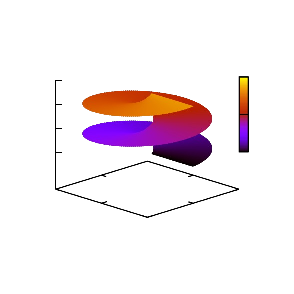
\includegraphics{log_riemann_imag}}%
    \gplfronttext
  \end{picture}%
\endgroup

  \end{frame}

  \begin{frame}
    \frametitle{The Quantum Pendulum}
    We consider the Lagrangian of a quantum particle in a cosine potential:
    \begin{align*}
      \mathcal L = \frac{1}{2}\dot\phi^2-(1-\cos(\phi))
    \end{align*}
    \begin{itemize}
    \item Equation of motion: $\ddot \phi = \sin(\theta),$
    \item Energy: $E = \frac{1}{2}\dot\phi^2+(1-\cos(\phi)).$
    \end{itemize}
    A solution of 0 energy reads:
    \begin{align*}
      \phi(t) = 4\arctan(\exp(t)).
    \end{align*}
  \end{frame}
  \begin{frame}
    \frametitle{Numerical analytic continuation of the Quantum pentulum}
    Real part:
    % GNUPLOT: LaTeX picture with Postscript
\begingroup
  \makeatletter
  \providecommand\color[2][]{%
    \GenericError{(gnuplot) \space\space\space\@spaces}{%
      Package color not loaded in conjunction with
      terminal option `colourtext'%
    }{See the gnuplot documentation for explanation.%
    }{Either use 'blacktext' in gnuplot or load the package
      color.sty in LaTeX.}%
    \renewcommand\color[2][]{}%
  }%
  \providecommand\includegraphics[2][]{%
    \GenericError{(gnuplot) \space\space\space\@spaces}{%
      Package graphicx or graphics not loaded%
    }{See the gnuplot documentation for explanation.%
    }{The gnuplot epslatex terminal needs graphicx.sty or graphics.sty.}%
    \renewcommand\includegraphics[2][]{}%
  }%
  \providecommand\rotatebox[2]{#2}%
  \@ifundefined{ifGPcolor}{%
    \newif\ifGPcolor
    \GPcolortrue
  }{}%
  \@ifundefined{ifGPblacktext}{%
    \newif\ifGPblacktext
    \GPblacktexttrue
  }{}%
  % define a \g@addto@macro without @ in the name:
  \let\gplgaddtomacro\g@addto@macro
  % define empty templates for all commands taking text:
  \gdef\gplbacktext{}%
  \gdef\gplfronttext{}%
  \makeatother
  \ifGPblacktext
    % no textcolor at all
    \def\colorrgb#1{}%
    \def\colorgray#1{}%
  \else
    % gray or color?
    \ifGPcolor
      \def\colorrgb#1{\color[rgb]{#1}}%
      \def\colorgray#1{\color[gray]{#1}}%
      \expandafter\def\csname LTw\endcsname{\color{white}}%
      \expandafter\def\csname LTb\endcsname{\color{black}}%
      \expandafter\def\csname LTa\endcsname{\color{black}}%
      \expandafter\def\csname LT0\endcsname{\color[rgb]{1,0,0}}%
      \expandafter\def\csname LT1\endcsname{\color[rgb]{0,1,0}}%
      \expandafter\def\csname LT2\endcsname{\color[rgb]{0,0,1}}%
      \expandafter\def\csname LT3\endcsname{\color[rgb]{1,0,1}}%
      \expandafter\def\csname LT4\endcsname{\color[rgb]{0,1,1}}%
      \expandafter\def\csname LT5\endcsname{\color[rgb]{1,1,0}}%
      \expandafter\def\csname LT6\endcsname{\color[rgb]{0,0,0}}%
      \expandafter\def\csname LT7\endcsname{\color[rgb]{1,0.3,0}}%
      \expandafter\def\csname LT8\endcsname{\color[rgb]{0.5,0.5,0.5}}%
    \else
      % gray
      \def\colorrgb#1{\color{black}}%
      \def\colorgray#1{\color[gray]{#1}}%
      \expandafter\def\csname LTw\endcsname{\color{white}}%
      \expandafter\def\csname LTb\endcsname{\color{black}}%
      \expandafter\def\csname LTa\endcsname{\color{black}}%
      \expandafter\def\csname LT0\endcsname{\color{black}}%
      \expandafter\def\csname LT1\endcsname{\color{black}}%
      \expandafter\def\csname LT2\endcsname{\color{black}}%
      \expandafter\def\csname LT3\endcsname{\color{black}}%
      \expandafter\def\csname LT4\endcsname{\color{black}}%
      \expandafter\def\csname LT5\endcsname{\color{black}}%
      \expandafter\def\csname LT6\endcsname{\color{black}}%
      \expandafter\def\csname LT7\endcsname{\color{black}}%
      \expandafter\def\csname LT8\endcsname{\color{black}}%
    \fi
  \fi
  \setlength{\unitlength}{0.0500bp}%
  \begin{picture}(6236.00,2834.00)%
    \gplgaddtomacro\gplbacktext{%
    }%
    \gplgaddtomacro\gplfronttext{%
      \csname LTb\endcsname%
      \put(1139,517){\makebox(0,0){\strut{}-9}}%
      \put(1799,517){\makebox(0,0){\strut{}-6}}%
      \put(2459,517){\makebox(0,0){\strut{}-3}}%
      \put(3118,517){\makebox(0,0){\strut{} 0}}%
      \put(3777,517){\makebox(0,0){\strut{} 3}}%
      \put(4437,517){\makebox(0,0){\strut{} 6}}%
      \put(5097,517){\makebox(0,0){\strut{} 9}}%
      \put(3118,187){\makebox(0,0){\strut{}$x$}}%
      \put(874,803){\makebox(0,0)[r]{\strut{} 0}}%
      \put(874,1264){\makebox(0,0)[r]{\strut{} 3}}%
      \put(874,1725){\makebox(0,0)[r]{\strut{} 6}}%
      \put(874,2186){\makebox(0,0)[r]{\strut{} 9}}%
      \put(544,1527){\rotatebox{-270}{\makebox(0,0){\strut{}$y$}}}%
      \put(5633,802){\makebox(0,0)[l]{\strut{} 0}}%
      \put(5633,1526){\makebox(0,0)[l]{\strut{} 6.28319}}%
      \put(5633,2251){\makebox(0,0)[l]{\strut{} 12.5664}}%
    }%
    \gplbacktext
    \put(0,0){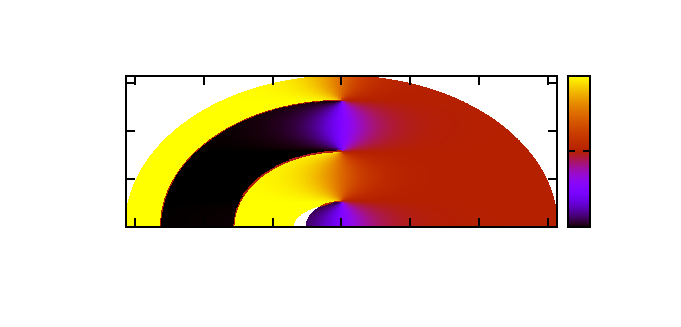
\includegraphics{sine_real}}%
    \gplfronttext
  \end{picture}%
\endgroup

  \end{frame}
  \begin{frame}
    \frametitle{Numerical analytic continuation of the Quantum pentulum}
    Imaginary part:
    % GNUPLOT: LaTeX picture with Postscript
\begingroup
  \makeatletter
  \providecommand\color[2][]{%
    \GenericError{(gnuplot) \space\space\space\@spaces}{%
      Package color not loaded in conjunction with
      terminal option `colourtext'%
    }{See the gnuplot documentation for explanation.%
    }{Either use 'blacktext' in gnuplot or load the package
      color.sty in LaTeX.}%
    \renewcommand\color[2][]{}%
  }%
  \providecommand\includegraphics[2][]{%
    \GenericError{(gnuplot) \space\space\space\@spaces}{%
      Package graphicx or graphics not loaded%
    }{See the gnuplot documentation for explanation.%
    }{The gnuplot epslatex terminal needs graphicx.sty or graphics.sty.}%
    \renewcommand\includegraphics[2][]{}%
  }%
  \providecommand\rotatebox[2]{#2}%
  \@ifundefined{ifGPcolor}{%
    \newif\ifGPcolor
    \GPcolortrue
  }{}%
  \@ifundefined{ifGPblacktext}{%
    \newif\ifGPblacktext
    \GPblacktexttrue
  }{}%
  % define a \g@addto@macro without @ in the name:
  \let\gplgaddtomacro\g@addto@macro
  % define empty templates for all commands taking text:
  \gdef\gplbacktext{}%
  \gdef\gplfronttext{}%
  \makeatother
  \ifGPblacktext
    % no textcolor at all
    \def\colorrgb#1{}%
    \def\colorgray#1{}%
  \else
    % gray or color?
    \ifGPcolor
      \def\colorrgb#1{\color[rgb]{#1}}%
      \def\colorgray#1{\color[gray]{#1}}%
      \expandafter\def\csname LTw\endcsname{\color{white}}%
      \expandafter\def\csname LTb\endcsname{\color{black}}%
      \expandafter\def\csname LTa\endcsname{\color{black}}%
      \expandafter\def\csname LT0\endcsname{\color[rgb]{1,0,0}}%
      \expandafter\def\csname LT1\endcsname{\color[rgb]{0,1,0}}%
      \expandafter\def\csname LT2\endcsname{\color[rgb]{0,0,1}}%
      \expandafter\def\csname LT3\endcsname{\color[rgb]{1,0,1}}%
      \expandafter\def\csname LT4\endcsname{\color[rgb]{0,1,1}}%
      \expandafter\def\csname LT5\endcsname{\color[rgb]{1,1,0}}%
      \expandafter\def\csname LT6\endcsname{\color[rgb]{0,0,0}}%
      \expandafter\def\csname LT7\endcsname{\color[rgb]{1,0.3,0}}%
      \expandafter\def\csname LT8\endcsname{\color[rgb]{0.5,0.5,0.5}}%
    \else
      % gray
      \def\colorrgb#1{\color{black}}%
      \def\colorgray#1{\color[gray]{#1}}%
      \expandafter\def\csname LTw\endcsname{\color{white}}%
      \expandafter\def\csname LTb\endcsname{\color{black}}%
      \expandafter\def\csname LTa\endcsname{\color{black}}%
      \expandafter\def\csname LT0\endcsname{\color{black}}%
      \expandafter\def\csname LT1\endcsname{\color{black}}%
      \expandafter\def\csname LT2\endcsname{\color{black}}%
      \expandafter\def\csname LT3\endcsname{\color{black}}%
      \expandafter\def\csname LT4\endcsname{\color{black}}%
      \expandafter\def\csname LT5\endcsname{\color{black}}%
      \expandafter\def\csname LT6\endcsname{\color{black}}%
      \expandafter\def\csname LT7\endcsname{\color{black}}%
      \expandafter\def\csname LT8\endcsname{\color{black}}%
    \fi
  \fi
  \setlength{\unitlength}{0.0500bp}%
  \begin{picture}(6236.00,2834.00)%
    \gplgaddtomacro\gplbacktext{%
    }%
    \gplgaddtomacro\gplfronttext{%
      \csname LTb\endcsname%
      \put(1139,517){\makebox(0,0){\strut{}-9}}%
      \put(1799,517){\makebox(0,0){\strut{}-6}}%
      \put(2459,517){\makebox(0,0){\strut{}-3}}%
      \put(3118,517){\makebox(0,0){\strut{} 0}}%
      \put(3777,517){\makebox(0,0){\strut{} 3}}%
      \put(4437,517){\makebox(0,0){\strut{} 6}}%
      \put(5097,517){\makebox(0,0){\strut{} 9}}%
      \put(3118,187){\makebox(0,0){\strut{}$x$}}%
      \put(874,803){\makebox(0,0)[r]{\strut{} 0}}%
      \put(874,1264){\makebox(0,0)[r]{\strut{} 3}}%
      \put(874,1725){\makebox(0,0)[r]{\strut{} 6}}%
      \put(874,2186){\makebox(0,0)[r]{\strut{} 9}}%
      \put(544,1527){\rotatebox{-270}{\makebox(0,0){\strut{}$y$}}}%
      \put(5633,802){\makebox(0,0)[l]{\strut{}-5}}%
      \put(5633,1526){\makebox(0,0)[l]{\strut{} 0}}%
      \put(5633,2251){\makebox(0,0)[l]{\strut{} 5}}%
    }%
    \gplbacktext
    \put(0,0){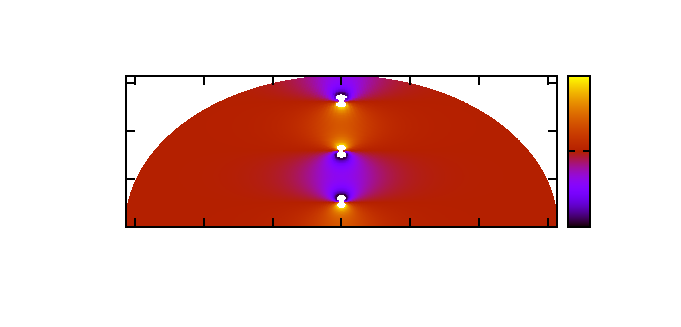
\includegraphics{sine_imag}}%
    \gplfronttext
  \end{picture}%
\endgroup

  \end{frame}


\end{section}

\begin{section}{Classical field theory situations}
  \begin{frame}
    \frametitle{Classical field theory situations}
    \begin{itemize}
    \item Abelian Vortex of a complex scalar in $(2+1)$ dimensions,
      with $U(1)$ gauge symmetry
    \item Non-Abelian Monopole of a real scalar triplet in $(3+1)$
      dimensions, with $SU(2)$ gauge symmetry. (Georgi-Glashow model)
    \end{itemize}
  \end{frame}

  \begin{frame}
    \frametitle{Abelian Vortex}
    The Lagrangian of the  theory reads:
    \begin{align*}
      \mathcal L = \frac{1}{2}\mathrm D_\mu\phi^*\mathrm D_\mu\phi-\frac{\lambda}{2}(\phi^*\phi-v^2)^2-\frac{1}{4}F_{\mu\nu}^2.
    \end{align*}
    \begin{itemize}
    \item Field equations:
      \begin{align*}
        &\partial^\nu F_{\nu\mu}=ie(\phi^*\mathrm D_\mu-\phi\mathrm D_\mu\phi^*),\\
        &\mathrm D^\mu\mathrm D_\mu\phi+\lambda(\phi^*\phi-v^2)\phi=0\ \&\ c.c. .
      \end{align*}
    \item Energy functional, static case:
      \begin{align*}
        E = 4\pi\int_0^\infty r^2\mathrm d r\left(\frac{1}{4}F_{ij}F_{ij}+\frac{1}{2}\mathrm D_i\phi\mathrm D_i\phi^*+\frac{\lambda}{2}(\phi^*\phi-v^2)^2\right).
      \end{align*}
    \end{itemize}
  \end{frame}
  \begin{frame}
    \frametitle{Static, Spherically symmetric ansatz} The simplest
    spherically symmetric static solution can be expressed with the
    ansatz:
    \begin{align*}
      &\phi(r,\theta) = ve^{i\theta}F(r),\\
      &A_i(r) = -\frac{1}{er}\varepsilon_{ij}n_jA(r).
    \end{align*}
    Leading to the equations for $f(a)$ and $a(r)$:
    \begin{align*}
      &-\frac{\mathrm d}{\mathrm d r}\left[\frac{1}{r}\frac{\mathrm d A}{\mathrm dr}\right] -2e^2v^2\frac{F^2(1-A)}{r} = 0,\\
      &-\frac{\mathrm d}{\mathrm d r}\left[r\frac{\mathrm d F}{\mathrm dr}\right] +\lambda v^2 r(F^2-1)F+\frac{F}{r}(A-1)^2 = 0.
    \end{align*}
  \end{frame}
  \begin{frame}
    \frametitle{Vortex profile}
    Higgs field:
    % GNUPLOT: LaTeX picture with Postscript
\begingroup
\scriptsize
  \makeatletter
  \providecommand\color[2][]{%
    \GenericError{(gnuplot) \space\space\space\@spaces}{%
      Package color not loaded in conjunction with
      terminal option `colourtext'%
    }{See the gnuplot documentation for explanation.%
    }{Either use 'blacktext' in gnuplot or load the package
      color.sty in LaTeX.}%
    \renewcommand\color[2][]{}%
  }%
  \providecommand\includegraphics[2][]{%
    \GenericError{(gnuplot) \space\space\space\@spaces}{%
      Package graphicx or graphics not loaded%
    }{See the gnuplot documentation for explanation.%
    }{The gnuplot epslatex terminal needs graphicx.sty or graphics.sty.}%
    \renewcommand\includegraphics[2][]{}%
  }%
  \providecommand\rotatebox[2]{#2}%
  \@ifundefined{ifGPcolor}{%
    \newif\ifGPcolor
    \GPcolortrue
  }{}%
  \@ifundefined{ifGPblacktext}{%
    \newif\ifGPblacktext
    \GPblacktexttrue
  }{}%
  % define a \g@addto@macro without @ in the name:
  \let\gplgaddtomacro\g@addto@macro
  % define empty templates for all commands taking text:
  \gdef\gplbacktext{}%
  \gdef\gplfronttext{}%
  \makeatother
  \ifGPblacktext
    % no textcolor at all
    \def\colorrgb#1{}%
    \def\colorgray#1{}%
  \else
    % gray or color?
    \ifGPcolor
      \def\colorrgb#1{\color[rgb]{#1}}%
      \def\colorgray#1{\color[gray]{#1}}%
      \expandafter\def\csname LTw\endcsname{\color{white}}%
      \expandafter\def\csname LTb\endcsname{\color{black}}%
      \expandafter\def\csname LTa\endcsname{\color{black}}%
      \expandafter\def\csname LT0\endcsname{\color[rgb]{1,0,0}}%
      \expandafter\def\csname LT1\endcsname{\color[rgb]{0,1,0}}%
      \expandafter\def\csname LT2\endcsname{\color[rgb]{0,0,1}}%
      \expandafter\def\csname LT3\endcsname{\color[rgb]{1,0,1}}%
      \expandafter\def\csname LT4\endcsname{\color[rgb]{0,1,1}}%
      \expandafter\def\csname LT5\endcsname{\color[rgb]{1,1,0}}%
      \expandafter\def\csname LT6\endcsname{\color[rgb]{0,0,0}}%
      \expandafter\def\csname LT7\endcsname{\color[rgb]{1,0.3,0}}%
      \expandafter\def\csname LT8\endcsname{\color[rgb]{0.5,0.5,0.5}}%
    \else
      % gray
      \def\colorrgb#1{\color{black}}%
      \def\colorgray#1{\color[gray]{#1}}%
      \expandafter\def\csname LTw\endcsname{\color{white}}%
      \expandafter\def\csname LTb\endcsname{\color{black}}%
      \expandafter\def\csname LTa\endcsname{\color{black}}%
      \expandafter\def\csname LT0\endcsname{\color{black}}%
      \expandafter\def\csname LT1\endcsname{\color{black}}%
      \expandafter\def\csname LT2\endcsname{\color{black}}%
      \expandafter\def\csname LT3\endcsname{\color{black}}%
      \expandafter\def\csname LT4\endcsname{\color{black}}%
      \expandafter\def\csname LT5\endcsname{\color{black}}%
      \expandafter\def\csname LT6\endcsname{\color{black}}%
      \expandafter\def\csname LT7\endcsname{\color{black}}%
      \expandafter\def\csname LT8\endcsname{\color{black}}%
    \fi
  \fi
  \setlength{\unitlength}{0.0500bp}%
  \begin{picture}(6236.00,2834.00)%
    \gplgaddtomacro\gplbacktext{%
      \csname LTb\endcsname%
      \put(946,704){\makebox(0,0)[r]{\strut{} 0}}%
      \put(946,1015){\makebox(0,0)[r]{\strut{} 0.2}}%
      \put(946,1326){\makebox(0,0)[r]{\strut{} 0.4}}%
      \put(946,1637){\makebox(0,0)[r]{\strut{} 0.6}}%
      \put(946,1947){\makebox(0,0)[r]{\strut{} 0.8}}%
      \put(946,2258){\makebox(0,0)[r]{\strut{} 1}}%
      \put(1078,484){\makebox(0,0){\strut{} 0}}%
      \put(2043,484){\makebox(0,0){\strut{} 2}}%
      \put(3009,484){\makebox(0,0){\strut{} 4}}%
      \put(3974,484){\makebox(0,0){\strut{} 6}}%
      \put(4940,484){\makebox(0,0){\strut{} 8}}%
      \put(5905,484){\makebox(0,0){\strut{} 10}}%
      \put(308,1636){\rotatebox{-270}{\makebox(0,0){\strut{}$F(r)$}}}%
      \put(3491,154){\makebox(0,0){\strut{}$r$}}%
    }%
    \gplgaddtomacro\gplfronttext{%
      \csname LTb\endcsname%
      \put(4918,1317){\makebox(0,0)[r]{\strut{}$\lambda=0.5$}}%
      \csname LTb\endcsname%
      \put(4918,1097){\makebox(0,0)[r]{\strut{}$\lambda=1$}}%
      \csname LTb\endcsname%
      \put(4918,877){\makebox(0,0)[r]{\strut{}$\lambda=2$}}%
    }%
    \gplbacktext
    \put(0,0){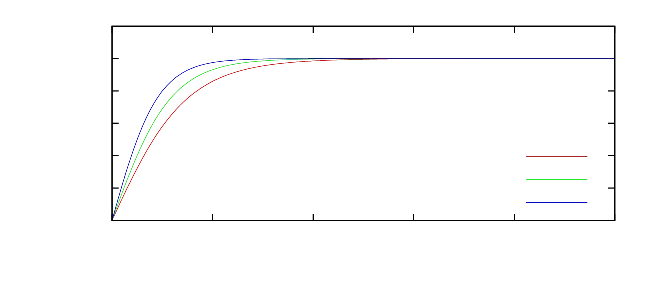
\includegraphics{vortex_func_f}}%
    \gplfronttext
  \end{picture}%
\endgroup

  \end{frame}

  \begin{frame}
    \frametitle{Vortex profile}
    Gauge Field:
    % GNUPLOT: LaTeX picture with Postscript
\begingroup
\scriptsize
  \makeatletter
  \providecommand\color[2][]{%
    \GenericError{(gnuplot) \space\space\space\@spaces}{%
      Package color not loaded in conjunction with
      terminal option `colourtext'%
    }{See the gnuplot documentation for explanation.%
    }{Either use 'blacktext' in gnuplot or load the package
      color.sty in LaTeX.}%
    \renewcommand\color[2][]{}%
  }%
  \providecommand\includegraphics[2][]{%
    \GenericError{(gnuplot) \space\space\space\@spaces}{%
      Package graphicx or graphics not loaded%
    }{See the gnuplot documentation for explanation.%
    }{The gnuplot epslatex terminal needs graphicx.sty or graphics.sty.}%
    \renewcommand\includegraphics[2][]{}%
  }%
  \providecommand\rotatebox[2]{#2}%
  \@ifundefined{ifGPcolor}{%
    \newif\ifGPcolor
    \GPcolortrue
  }{}%
  \@ifundefined{ifGPblacktext}{%
    \newif\ifGPblacktext
    \GPblacktexttrue
  }{}%
  % define a \g@addto@macro without @ in the name:
  \let\gplgaddtomacro\g@addto@macro
  % define empty templates for all commands taking text:
  \gdef\gplbacktext{}%
  \gdef\gplfronttext{}%
  \makeatother
  \ifGPblacktext
    % no textcolor at all
    \def\colorrgb#1{}%
    \def\colorgray#1{}%
  \else
    % gray or color?
    \ifGPcolor
      \def\colorrgb#1{\color[rgb]{#1}}%
      \def\colorgray#1{\color[gray]{#1}}%
      \expandafter\def\csname LTw\endcsname{\color{white}}%
      \expandafter\def\csname LTb\endcsname{\color{black}}%
      \expandafter\def\csname LTa\endcsname{\color{black}}%
      \expandafter\def\csname LT0\endcsname{\color[rgb]{1,0,0}}%
      \expandafter\def\csname LT1\endcsname{\color[rgb]{0,1,0}}%
      \expandafter\def\csname LT2\endcsname{\color[rgb]{0,0,1}}%
      \expandafter\def\csname LT3\endcsname{\color[rgb]{1,0,1}}%
      \expandafter\def\csname LT4\endcsname{\color[rgb]{0,1,1}}%
      \expandafter\def\csname LT5\endcsname{\color[rgb]{1,1,0}}%
      \expandafter\def\csname LT6\endcsname{\color[rgb]{0,0,0}}%
      \expandafter\def\csname LT7\endcsname{\color[rgb]{1,0.3,0}}%
      \expandafter\def\csname LT8\endcsname{\color[rgb]{0.5,0.5,0.5}}%
    \else
      % gray
      \def\colorrgb#1{\color{black}}%
      \def\colorgray#1{\color[gray]{#1}}%
      \expandafter\def\csname LTw\endcsname{\color{white}}%
      \expandafter\def\csname LTb\endcsname{\color{black}}%
      \expandafter\def\csname LTa\endcsname{\color{black}}%
      \expandafter\def\csname LT0\endcsname{\color{black}}%
      \expandafter\def\csname LT1\endcsname{\color{black}}%
      \expandafter\def\csname LT2\endcsname{\color{black}}%
      \expandafter\def\csname LT3\endcsname{\color{black}}%
      \expandafter\def\csname LT4\endcsname{\color{black}}%
      \expandafter\def\csname LT5\endcsname{\color{black}}%
      \expandafter\def\csname LT6\endcsname{\color{black}}%
      \expandafter\def\csname LT7\endcsname{\color{black}}%
      \expandafter\def\csname LT8\endcsname{\color{black}}%
    \fi
  \fi
  \setlength{\unitlength}{0.0500bp}%
  \begin{picture}(6236.00,2834.00)%
    \gplgaddtomacro\gplbacktext{%
      \csname LTb\endcsname%
      \put(946,704){\makebox(0,0)[r]{\strut{} 0}}%
      \put(946,1015){\makebox(0,0)[r]{\strut{} 0.2}}%
      \put(946,1326){\makebox(0,0)[r]{\strut{} 0.4}}%
      \put(946,1637){\makebox(0,0)[r]{\strut{} 0.6}}%
      \put(946,1947){\makebox(0,0)[r]{\strut{} 0.8}}%
      \put(946,2258){\makebox(0,0)[r]{\strut{} 1}}%
      \put(1078,484){\makebox(0,0){\strut{} 0}}%
      \put(2043,484){\makebox(0,0){\strut{} 2}}%
      \put(3009,484){\makebox(0,0){\strut{} 4}}%
      \put(3974,484){\makebox(0,0){\strut{} 6}}%
      \put(4940,484){\makebox(0,0){\strut{} 8}}%
      \put(5905,484){\makebox(0,0){\strut{} 10}}%
      \put(308,1636){\rotatebox{-270}{\makebox(0,0){\strut{}$A(f)$}}}%
      \put(3491,154){\makebox(0,0){\strut{}$r$}}%
    }%
    \gplgaddtomacro\gplfronttext{%
      \csname LTb\endcsname%
      \put(4918,1317){\makebox(0,0)[r]{\strut{}$\lambda=0.5$}}%
      \csname LTb\endcsname%
      \put(4918,1097){\makebox(0,0)[r]{\strut{}$\lambda=1$}}%
      \csname LTb\endcsname%
      \put(4918,877){\makebox(0,0)[r]{\strut{}$\lambda=2$}}%
    }%
    \gplbacktext
    \put(0,0){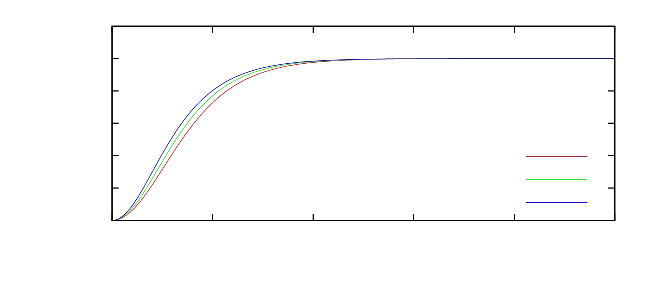
\includegraphics{vortex_func_a}}%
    \gplfronttext
  \end{picture}%
\endgroup

  \end{frame}

  \begin{frame}
    \frametitle{Analytic continuation of the Vortex}
    Real part of the Higgs field:
    % GNUPLOT: LaTeX picture with Postscript
\begingroup
\scriptsize
  \makeatletter
  \providecommand\color[2][]{%
    \GenericError{(gnuplot) \space\space\space\@spaces}{%
      Package color not loaded in conjunction with
      terminal option `colourtext'%
    }{See the gnuplot documentation for explanation.%
    }{Either use 'blacktext' in gnuplot or load the package
      color.sty in LaTeX.}%
    \renewcommand\color[2][]{}%
  }%
  \providecommand\includegraphics[2][]{%
    \GenericError{(gnuplot) \space\space\space\@spaces}{%
      Package graphicx or graphics not loaded%
    }{See the gnuplot documentation for explanation.%
    }{The gnuplot epslatex terminal needs graphicx.sty or graphics.sty.}%
    \renewcommand\includegraphics[2][]{}%
  }%
  \providecommand\rotatebox[2]{#2}%
  \@ifundefined{ifGPcolor}{%
    \newif\ifGPcolor
    \GPcolortrue
  }{}%
  \@ifundefined{ifGPblacktext}{%
    \newif\ifGPblacktext
    \GPblacktexttrue
  }{}%
  % define a \g@addto@macro without @ in the name:
  \let\gplgaddtomacro\g@addto@macro
  % define empty templates for all commands taking text:
  \gdef\gplbacktext{}%
  \gdef\gplfronttext{}%
  \makeatother
  \ifGPblacktext
    % no textcolor at all
    \def\colorrgb#1{}%
    \def\colorgray#1{}%
  \else
    % gray or color?
    \ifGPcolor
      \def\colorrgb#1{\color[rgb]{#1}}%
      \def\colorgray#1{\color[gray]{#1}}%
      \expandafter\def\csname LTw\endcsname{\color{white}}%
      \expandafter\def\csname LTb\endcsname{\color{black}}%
      \expandafter\def\csname LTa\endcsname{\color{black}}%
      \expandafter\def\csname LT0\endcsname{\color[rgb]{1,0,0}}%
      \expandafter\def\csname LT1\endcsname{\color[rgb]{0,1,0}}%
      \expandafter\def\csname LT2\endcsname{\color[rgb]{0,0,1}}%
      \expandafter\def\csname LT3\endcsname{\color[rgb]{1,0,1}}%
      \expandafter\def\csname LT4\endcsname{\color[rgb]{0,1,1}}%
      \expandafter\def\csname LT5\endcsname{\color[rgb]{1,1,0}}%
      \expandafter\def\csname LT6\endcsname{\color[rgb]{0,0,0}}%
      \expandafter\def\csname LT7\endcsname{\color[rgb]{1,0.3,0}}%
      \expandafter\def\csname LT8\endcsname{\color[rgb]{0.5,0.5,0.5}}%
    \else
      % gray
      \def\colorrgb#1{\color{black}}%
      \def\colorgray#1{\color[gray]{#1}}%
      \expandafter\def\csname LTw\endcsname{\color{white}}%
      \expandafter\def\csname LTb\endcsname{\color{black}}%
      \expandafter\def\csname LTa\endcsname{\color{black}}%
      \expandafter\def\csname LT0\endcsname{\color{black}}%
      \expandafter\def\csname LT1\endcsname{\color{black}}%
      \expandafter\def\csname LT2\endcsname{\color{black}}%
      \expandafter\def\csname LT3\endcsname{\color{black}}%
      \expandafter\def\csname LT4\endcsname{\color{black}}%
      \expandafter\def\csname LT5\endcsname{\color{black}}%
      \expandafter\def\csname LT6\endcsname{\color{black}}%
      \expandafter\def\csname LT7\endcsname{\color{black}}%
      \expandafter\def\csname LT8\endcsname{\color{black}}%
    \fi
  \fi
  \setlength{\unitlength}{0.0500bp}%
  \begin{picture}(6236.00,2834.00)%
    \gplgaddtomacro\gplbacktext{%
    }%
    \gplgaddtomacro\gplfronttext{%
      \csname LTb\endcsname%
      \put(1046,517){\makebox(0,0){\strut{}-10}}%
      \put(2082,517){\makebox(0,0){\strut{}-5}}%
      \put(3118,517){\makebox(0,0){\strut{} 0}}%
      \put(4154,517){\makebox(0,0){\strut{} 5}}%
      \put(5190,517){\makebox(0,0){\strut{} 10}}%
      \put(3118,187){\makebox(0,0){\strut{}$x$}}%
      \put(874,803){\makebox(0,0)[r]{\strut{} 0}}%
      \put(874,1527){\makebox(0,0)[r]{\strut{} 5}}%
      \put(874,2251){\makebox(0,0)[r]{\strut{} 10}}%
      \put(544,1527){\rotatebox{-270}{\makebox(0,0){\strut{}$y$}}}%
      \put(5633,836){\makebox(0,0)[l]{\strut{}-2}}%
      \put(5633,1526){\makebox(0,0)[l]{\strut{} 0}}%
      \put(5633,2216){\makebox(0,0)[l]{\strut{} 2}}%
    }%
    \gplbacktext
    \put(0,0){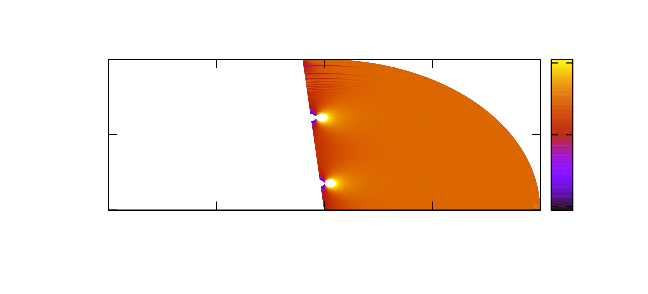
\includegraphics{vortex_anal_f_real}}%
    \gplfronttext
  \end{picture}%
\endgroup

  \end{frame}

  \begin{frame}
    \frametitle{Analytic continuation of the Vortex}
    Real part of the gauge field:
    % GNUPLOT: LaTeX picture with Postscript
\begingroup
\scriptsize
  \makeatletter
  \providecommand\color[2][]{%
    \GenericError{(gnuplot) \space\space\space\@spaces}{%
      Package color not loaded in conjunction with
      terminal option `colourtext'%
    }{See the gnuplot documentation for explanation.%
    }{Either use 'blacktext' in gnuplot or load the package
      color.sty in LaTeX.}%
    \renewcommand\color[2][]{}%
  }%
  \providecommand\includegraphics[2][]{%
    \GenericError{(gnuplot) \space\space\space\@spaces}{%
      Package graphicx or graphics not loaded%
    }{See the gnuplot documentation for explanation.%
    }{The gnuplot epslatex terminal needs graphicx.sty or graphics.sty.}%
    \renewcommand\includegraphics[2][]{}%
  }%
  \providecommand\rotatebox[2]{#2}%
  \@ifundefined{ifGPcolor}{%
    \newif\ifGPcolor
    \GPcolortrue
  }{}%
  \@ifundefined{ifGPblacktext}{%
    \newif\ifGPblacktext
    \GPblacktexttrue
  }{}%
  % define a \g@addto@macro without @ in the name:
  \let\gplgaddtomacro\g@addto@macro
  % define empty templates for all commands taking text:
  \gdef\gplbacktext{}%
  \gdef\gplfronttext{}%
  \makeatother
  \ifGPblacktext
    % no textcolor at all
    \def\colorrgb#1{}%
    \def\colorgray#1{}%
  \else
    % gray or color?
    \ifGPcolor
      \def\colorrgb#1{\color[rgb]{#1}}%
      \def\colorgray#1{\color[gray]{#1}}%
      \expandafter\def\csname LTw\endcsname{\color{white}}%
      \expandafter\def\csname LTb\endcsname{\color{black}}%
      \expandafter\def\csname LTa\endcsname{\color{black}}%
      \expandafter\def\csname LT0\endcsname{\color[rgb]{1,0,0}}%
      \expandafter\def\csname LT1\endcsname{\color[rgb]{0,1,0}}%
      \expandafter\def\csname LT2\endcsname{\color[rgb]{0,0,1}}%
      \expandafter\def\csname LT3\endcsname{\color[rgb]{1,0,1}}%
      \expandafter\def\csname LT4\endcsname{\color[rgb]{0,1,1}}%
      \expandafter\def\csname LT5\endcsname{\color[rgb]{1,1,0}}%
      \expandafter\def\csname LT6\endcsname{\color[rgb]{0,0,0}}%
      \expandafter\def\csname LT7\endcsname{\color[rgb]{1,0.3,0}}%
      \expandafter\def\csname LT8\endcsname{\color[rgb]{0.5,0.5,0.5}}%
    \else
      % gray
      \def\colorrgb#1{\color{black}}%
      \def\colorgray#1{\color[gray]{#1}}%
      \expandafter\def\csname LTw\endcsname{\color{white}}%
      \expandafter\def\csname LTb\endcsname{\color{black}}%
      \expandafter\def\csname LTa\endcsname{\color{black}}%
      \expandafter\def\csname LT0\endcsname{\color{black}}%
      \expandafter\def\csname LT1\endcsname{\color{black}}%
      \expandafter\def\csname LT2\endcsname{\color{black}}%
      \expandafter\def\csname LT3\endcsname{\color{black}}%
      \expandafter\def\csname LT4\endcsname{\color{black}}%
      \expandafter\def\csname LT5\endcsname{\color{black}}%
      \expandafter\def\csname LT6\endcsname{\color{black}}%
      \expandafter\def\csname LT7\endcsname{\color{black}}%
      \expandafter\def\csname LT8\endcsname{\color{black}}%
    \fi
  \fi
  \setlength{\unitlength}{0.0500bp}%
  \begin{picture}(6236.00,2834.00)%
    \gplgaddtomacro\gplbacktext{%
    }%
    \gplgaddtomacro\gplfronttext{%
      \csname LTb\endcsname%
      \put(1046,517){\makebox(0,0){\strut{}-10}}%
      \put(2082,517){\makebox(0,0){\strut{}-5}}%
      \put(3118,517){\makebox(0,0){\strut{} 0}}%
      \put(4154,517){\makebox(0,0){\strut{} 5}}%
      \put(5190,517){\makebox(0,0){\strut{} 10}}%
      \put(3118,187){\makebox(0,0){\strut{}$x$}}%
      \put(874,803){\makebox(0,0)[r]{\strut{} 0}}%
      \put(874,1527){\makebox(0,0)[r]{\strut{} 5}}%
      \put(874,2251){\makebox(0,0)[r]{\strut{} 10}}%
      \put(544,1527){\rotatebox{-270}{\makebox(0,0){\strut{}$y$}}}%
      \put(5633,816){\makebox(0,0)[l]{\strut{}-5}}%
      \put(5633,1526){\makebox(0,0)[l]{\strut{} 0}}%
      \put(5633,2236){\makebox(0,0)[l]{\strut{} 5}}%
    }%
    \gplbacktext
    \put(0,0){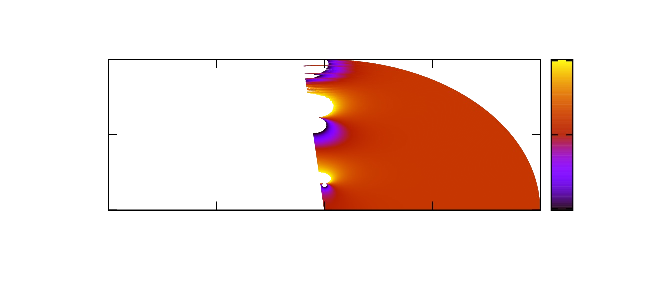
\includegraphics{vortex_anal_a_real}}%
    \gplfronttext
  \end{picture}%
\endgroup

  \end{frame}

  \begin{frame}
    \frametitle{Non-Abelian Monopole}
    The Lagrangian of the  theory reads:
    \begin{align*}
      \mathcal L = \frac{1}{2}\mathrm D_\mu\phi^a\mathrm D_\mu\phi^a-\frac{\lambda}{2}(\phi^a\phi^a-v^2)^2-\frac{1}{4}F_{\mu\nu}^aF_{\mu\nu}^a.
    \end{align*}
    \begin{itemize}
    \item Field equations:
      \begin{align*}
        &\mathrm D_\mu\mathrm D_\mu\phi^a+\lambda\phi^a(\phi^b\phi^b-v^2) = 0,\\
        &\partial^\nu F^a_{\nu\mu}=g\varepsilon^{abc}(A_\nu^bF_\mu^{c,\nu}+\mathrm D_\mu\phi^b\phi^c).
      \end{align*}
    \item Energy functional, static case:
      \begin{align*}
        E=4\pi\int_0^\infty r^2\mathrm dr\left(\frac{1}{4}F_{ij}^aF_{ij}^a+\frac{1}{2}\mathrm D_i\phi^a\mathrm D_i\phi^a +\frac{\lambda}{4}(\phi^a\phi^a-v^2)^2\right).
      \end{align*}
    \end{itemize}
  \end{frame}
  \begin{frame}
    \frametitle{'t Hooft--Polyakov ansatz} The first non-trivial
    static field configuration was proposed by 't Hooft \& Polyakof:
    \begin{align*}
      \left\{
      \begin{aligned}
        &\phi^a(r,\theta) = vn^ah(r),\\
        &A^a_i(r) = \frac{1}{gr^2}\varepsilon^{aij}n_j(1-f(r)),\ A_0^a = 0.
      \end{aligned}
      \right.
    \end{align*}
    Which lead to the field equations for $f(r)$ and $h(r)$:
    \begin{align*}
      &r^2h''=2hf^2+\lambda v^2 h(h^2-r^2),\\
      &r^2f''=f(f^2-1)-gv^2h^2f.
    \end{align*}
  \end{frame}
  \begin{frame}
    \frametitle{Bogomol'nyi--Prasad--Sommerfield limit} If we set the Higgs coupling constant to
    zero, the solution can be expressed in a simple form:
    \begin{align*}
      f(r) = \frac{r}{\sinh(r)}\quad;\quad h(r) = \sqrt{gv^2}(r\mathrm{coth}(r)-1).
    \end{align*}
  \end{frame}

  \begin{frame}
    \frametitle{Monopole profile}
    Higgs field profiled:
    % GNUPLOT: LaTeX picture with Postscript
\begingroup
  \makeatletter
  \providecommand\color[2][]{%
    \GenericError{(gnuplot) \space\space\space\@spaces}{%
      Package color not loaded in conjunction with
      terminal option `colourtext'%
    }{See the gnuplot documentation for explanation.%
    }{Either use 'blacktext' in gnuplot or load the package
      color.sty in LaTeX.}%
    \renewcommand\color[2][]{}%
  }%
  \providecommand\includegraphics[2][]{%
    \GenericError{(gnuplot) \space\space\space\@spaces}{%
      Package graphicx or graphics not loaded%
    }{See the gnuplot documentation for explanation.%
    }{The gnuplot epslatex terminal needs graphicx.sty or graphics.sty.}%
    \renewcommand\includegraphics[2][]{}%
  }%
  \providecommand\rotatebox[2]{#2}%
  \@ifundefined{ifGPcolor}{%
    \newif\ifGPcolor
    \GPcolortrue
  }{}%
  \@ifundefined{ifGPblacktext}{%
    \newif\ifGPblacktext
    \GPblacktexttrue
  }{}%
  % define a \g@addto@macro without @ in the name:
  \let\gplgaddtomacro\g@addto@macro
  % define empty templates for all commands taking text:
  \gdef\gplbacktext{}%
  \gdef\gplfronttext{}%
  \makeatother
  \ifGPblacktext
    % no textcolor at all
    \def\colorrgb#1{}%
    \def\colorgray#1{}%
  \else
    % gray or color?
    \ifGPcolor
      \def\colorrgb#1{\color[rgb]{#1}}%
      \def\colorgray#1{\color[gray]{#1}}%
      \expandafter\def\csname LTw\endcsname{\color{white}}%
      \expandafter\def\csname LTb\endcsname{\color{black}}%
      \expandafter\def\csname LTa\endcsname{\color{black}}%
      \expandafter\def\csname LT0\endcsname{\color[rgb]{1,0,0}}%
      \expandafter\def\csname LT1\endcsname{\color[rgb]{0,1,0}}%
      \expandafter\def\csname LT2\endcsname{\color[rgb]{0,0,1}}%
      \expandafter\def\csname LT3\endcsname{\color[rgb]{1,0,1}}%
      \expandafter\def\csname LT4\endcsname{\color[rgb]{0,1,1}}%
      \expandafter\def\csname LT5\endcsname{\color[rgb]{1,1,0}}%
      \expandafter\def\csname LT6\endcsname{\color[rgb]{0,0,0}}%
      \expandafter\def\csname LT7\endcsname{\color[rgb]{1,0.3,0}}%
      \expandafter\def\csname LT8\endcsname{\color[rgb]{0.5,0.5,0.5}}%
    \else
      % gray
      \def\colorrgb#1{\color{black}}%
      \def\colorgray#1{\color[gray]{#1}}%
      \expandafter\def\csname LTw\endcsname{\color{white}}%
      \expandafter\def\csname LTb\endcsname{\color{black}}%
      \expandafter\def\csname LTa\endcsname{\color{black}}%
      \expandafter\def\csname LT0\endcsname{\color{black}}%
      \expandafter\def\csname LT1\endcsname{\color{black}}%
      \expandafter\def\csname LT2\endcsname{\color{black}}%
      \expandafter\def\csname LT3\endcsname{\color{black}}%
      \expandafter\def\csname LT4\endcsname{\color{black}}%
      \expandafter\def\csname LT5\endcsname{\color{black}}%
      \expandafter\def\csname LT6\endcsname{\color{black}}%
      \expandafter\def\csname LT7\endcsname{\color{black}}%
      \expandafter\def\csname LT8\endcsname{\color{black}}%
    \fi
  \fi
  \setlength{\unitlength}{0.0500bp}%
  \begin{picture}(6236.00,2834.00)%
    \gplgaddtomacro\gplbacktext{%
      \csname LTb\endcsname%
      \put(1078,704){\makebox(0,0)[r]{\strut{} 0}}%
      \put(1078,1015){\makebox(0,0)[r]{\strut{} 0.2}}%
      \put(1078,1326){\makebox(0,0)[r]{\strut{} 0.4}}%
      \put(1078,1637){\makebox(0,0)[r]{\strut{} 0.6}}%
      \put(1078,1947){\makebox(0,0)[r]{\strut{} 0.8}}%
      \put(1078,2258){\makebox(0,0)[r]{\strut{} 1}}%
      \put(1210,484){\makebox(0,0){\strut{} 0}}%
      \put(1881,484){\makebox(0,0){\strut{} 1}}%
      \put(2551,484){\makebox(0,0){\strut{} 2}}%
      \put(3222,484){\makebox(0,0){\strut{} 3}}%
      \put(3893,484){\makebox(0,0){\strut{} 4}}%
      \put(4564,484){\makebox(0,0){\strut{} 5}}%
      \put(5234,484){\makebox(0,0){\strut{} 6}}%
      \put(5905,484){\makebox(0,0){\strut{} 7}}%
      \put(308,1636){\rotatebox{-270}{\makebox(0,0){\strut{}$ f(r)$}}}%
      \put(3557,154){\makebox(0,0){\strut{}$r$}}%
    }%
    \gplgaddtomacro\gplfronttext{%
      \csname LTb\endcsname%
      \put(4918,1317){\makebox(0,0)[r]{\strut{}$\lambda=0$}}%
      \csname LTb\endcsname%
      \put(4918,1097){\makebox(0,0)[r]{\strut{}$\lambda=0.5$}}%
      \csname LTb\endcsname%
      \put(4918,877){\makebox(0,0)[r]{\strut{}$\lambda=1$}}%
    }%
    \gplbacktext
    \put(0,0){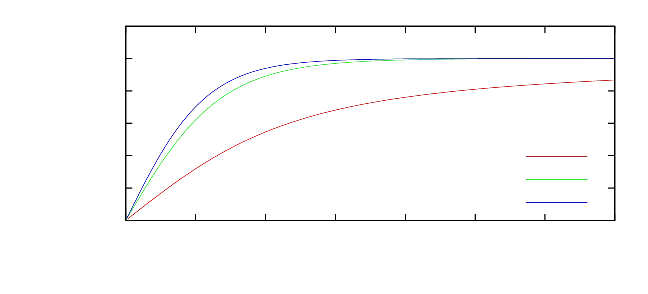
\includegraphics{monopole_funcs_f}}%
    \gplfronttext
  \end{picture}%
\endgroup

  \end{frame}

  \begin{frame}
    \frametitle{Monopole profile}
    Gauge field profile:
    % GNUPLOT: LaTeX picture with Postscript
\begingroup
  \makeatletter
  \providecommand\color[2][]{%
    \GenericError{(gnuplot) \space\space\space\@spaces}{%
      Package color not loaded in conjunction with
      terminal option `colourtext'%
    }{See the gnuplot documentation for explanation.%
    }{Either use 'blacktext' in gnuplot or load the package
      color.sty in LaTeX.}%
    \renewcommand\color[2][]{}%
  }%
  \providecommand\includegraphics[2][]{%
    \GenericError{(gnuplot) \space\space\space\@spaces}{%
      Package graphicx or graphics not loaded%
    }{See the gnuplot documentation for explanation.%
    }{The gnuplot epslatex terminal needs graphicx.sty or graphics.sty.}%
    \renewcommand\includegraphics[2][]{}%
  }%
  \providecommand\rotatebox[2]{#2}%
  \@ifundefined{ifGPcolor}{%
    \newif\ifGPcolor
    \GPcolortrue
  }{}%
  \@ifundefined{ifGPblacktext}{%
    \newif\ifGPblacktext
    \GPblacktexttrue
  }{}%
  % define a \g@addto@macro without @ in the name:
  \let\gplgaddtomacro\g@addto@macro
  % define empty templates for all commands taking text:
  \gdef\gplbacktext{}%
  \gdef\gplfronttext{}%
  \makeatother
  \ifGPblacktext
    % no textcolor at all
    \def\colorrgb#1{}%
    \def\colorgray#1{}%
  \else
    % gray or color?
    \ifGPcolor
      \def\colorrgb#1{\color[rgb]{#1}}%
      \def\colorgray#1{\color[gray]{#1}}%
      \expandafter\def\csname LTw\endcsname{\color{white}}%
      \expandafter\def\csname LTb\endcsname{\color{black}}%
      \expandafter\def\csname LTa\endcsname{\color{black}}%
      \expandafter\def\csname LT0\endcsname{\color[rgb]{1,0,0}}%
      \expandafter\def\csname LT1\endcsname{\color[rgb]{0,1,0}}%
      \expandafter\def\csname LT2\endcsname{\color[rgb]{0,0,1}}%
      \expandafter\def\csname LT3\endcsname{\color[rgb]{1,0,1}}%
      \expandafter\def\csname LT4\endcsname{\color[rgb]{0,1,1}}%
      \expandafter\def\csname LT5\endcsname{\color[rgb]{1,1,0}}%
      \expandafter\def\csname LT6\endcsname{\color[rgb]{0,0,0}}%
      \expandafter\def\csname LT7\endcsname{\color[rgb]{1,0.3,0}}%
      \expandafter\def\csname LT8\endcsname{\color[rgb]{0.5,0.5,0.5}}%
    \else
      % gray
      \def\colorrgb#1{\color{black}}%
      \def\colorgray#1{\color[gray]{#1}}%
      \expandafter\def\csname LTw\endcsname{\color{white}}%
      \expandafter\def\csname LTb\endcsname{\color{black}}%
      \expandafter\def\csname LTa\endcsname{\color{black}}%
      \expandafter\def\csname LT0\endcsname{\color{black}}%
      \expandafter\def\csname LT1\endcsname{\color{black}}%
      \expandafter\def\csname LT2\endcsname{\color{black}}%
      \expandafter\def\csname LT3\endcsname{\color{black}}%
      \expandafter\def\csname LT4\endcsname{\color{black}}%
      \expandafter\def\csname LT5\endcsname{\color{black}}%
      \expandafter\def\csname LT6\endcsname{\color{black}}%
      \expandafter\def\csname LT7\endcsname{\color{black}}%
      \expandafter\def\csname LT8\endcsname{\color{black}}%
    \fi
  \fi
  \setlength{\unitlength}{0.0500bp}%
  \begin{picture}(6236.00,2834.00)%
    \gplgaddtomacro\gplbacktext{%
      \csname LTb\endcsname%
      \put(1078,704){\makebox(0,0)[r]{\strut{} 0}}%
      \put(1078,1015){\makebox(0,0)[r]{\strut{} 0.2}}%
      \put(1078,1326){\makebox(0,0)[r]{\strut{} 0.4}}%
      \put(1078,1637){\makebox(0,0)[r]{\strut{} 0.6}}%
      \put(1078,1947){\makebox(0,0)[r]{\strut{} 0.8}}%
      \put(1078,2258){\makebox(0,0)[r]{\strut{} 1}}%
      \put(1210,484){\makebox(0,0){\strut{} 0}}%
      \put(1881,484){\makebox(0,0){\strut{} 1}}%
      \put(2551,484){\makebox(0,0){\strut{} 2}}%
      \put(3222,484){\makebox(0,0){\strut{} 3}}%
      \put(3893,484){\makebox(0,0){\strut{} 4}}%
      \put(4564,484){\makebox(0,0){\strut{} 5}}%
      \put(5234,484){\makebox(0,0){\strut{} 6}}%
      \put(5905,484){\makebox(0,0){\strut{} 7}}%
      \put(308,1636){\rotatebox{-270}{\makebox(0,0){\strut{}$N(r)\equiv 1-f(r)$}}}%
      \put(3557,154){\makebox(0,0){\strut{}$r$}}%
    }%
    \gplgaddtomacro\gplfronttext{%
      \csname LTb\endcsname%
      \put(4918,2396){\makebox(0,0)[r]{\strut{}$\lambda=0$}}%
      \csname LTb\endcsname%
      \put(4918,2176){\makebox(0,0)[r]{\strut{}$\lambda=0.5$}}%
      \csname LTb\endcsname%
      \put(4918,1956){\makebox(0,0)[r]{\strut{}$\lambda=1$}}%
    }%
    \gplbacktext
    \put(0,0){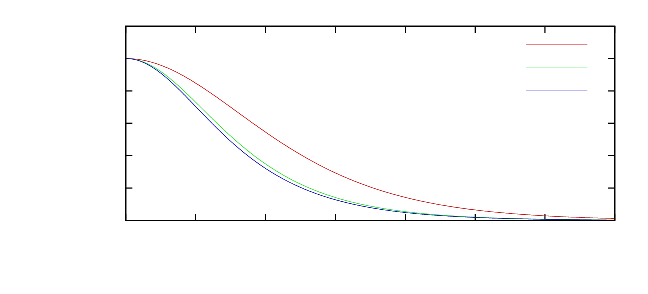
\includegraphics{monopole_funcs_a}}%
    \gplfronttext
  \end{picture}%
\endgroup

  \end{frame}

  \begin{frame}
    \frametitle{Analytic continuation of the Monopole}
    Real part of the Higgs field:
    % GNUPLOT: LaTeX picture with Postscript
\begingroup
  \makeatletter
  \providecommand\color[2][]{%
    \GenericError{(gnuplot) \space\space\space\@spaces}{%
      Package color not loaded in conjunction with
      terminal option `colourtext'%
    }{See the gnuplot documentation for explanation.%
    }{Either use 'blacktext' in gnuplot or load the package
      color.sty in LaTeX.}%
    \renewcommand\color[2][]{}%
  }%
  \providecommand\includegraphics[2][]{%
    \GenericError{(gnuplot) \space\space\space\@spaces}{%
      Package graphicx or graphics not loaded%
    }{See the gnuplot documentation for explanation.%
    }{The gnuplot epslatex terminal needs graphicx.sty or graphics.sty.}%
    \renewcommand\includegraphics[2][]{}%
  }%
  \providecommand\rotatebox[2]{#2}%
  \@ifundefined{ifGPcolor}{%
    \newif\ifGPcolor
    \GPcolortrue
  }{}%
  \@ifundefined{ifGPblacktext}{%
    \newif\ifGPblacktext
    \GPblacktexttrue
  }{}%
  % define a \g@addto@macro without @ in the name:
  \let\gplgaddtomacro\g@addto@macro
  % define empty templates for all commands taking text:
  \gdef\gplbacktext{}%
  \gdef\gplfronttext{}%
  \makeatother
  \ifGPblacktext
    % no textcolor at all
    \def\colorrgb#1{}%
    \def\colorgray#1{}%
  \else
    % gray or color?
    \ifGPcolor
      \def\colorrgb#1{\color[rgb]{#1}}%
      \def\colorgray#1{\color[gray]{#1}}%
      \expandafter\def\csname LTw\endcsname{\color{white}}%
      \expandafter\def\csname LTb\endcsname{\color{black}}%
      \expandafter\def\csname LTa\endcsname{\color{black}}%
      \expandafter\def\csname LT0\endcsname{\color[rgb]{1,0,0}}%
      \expandafter\def\csname LT1\endcsname{\color[rgb]{0,1,0}}%
      \expandafter\def\csname LT2\endcsname{\color[rgb]{0,0,1}}%
      \expandafter\def\csname LT3\endcsname{\color[rgb]{1,0,1}}%
      \expandafter\def\csname LT4\endcsname{\color[rgb]{0,1,1}}%
      \expandafter\def\csname LT5\endcsname{\color[rgb]{1,1,0}}%
      \expandafter\def\csname LT6\endcsname{\color[rgb]{0,0,0}}%
      \expandafter\def\csname LT7\endcsname{\color[rgb]{1,0.3,0}}%
      \expandafter\def\csname LT8\endcsname{\color[rgb]{0.5,0.5,0.5}}%
    \else
      % gray
      \def\colorrgb#1{\color{black}}%
      \def\colorgray#1{\color[gray]{#1}}%
      \expandafter\def\csname LTw\endcsname{\color{white}}%
      \expandafter\def\csname LTb\endcsname{\color{black}}%
      \expandafter\def\csname LTa\endcsname{\color{black}}%
      \expandafter\def\csname LT0\endcsname{\color{black}}%
      \expandafter\def\csname LT1\endcsname{\color{black}}%
      \expandafter\def\csname LT2\endcsname{\color{black}}%
      \expandafter\def\csname LT3\endcsname{\color{black}}%
      \expandafter\def\csname LT4\endcsname{\color{black}}%
      \expandafter\def\csname LT5\endcsname{\color{black}}%
      \expandafter\def\csname LT6\endcsname{\color{black}}%
      \expandafter\def\csname LT7\endcsname{\color{black}}%
      \expandafter\def\csname LT8\endcsname{\color{black}}%
    \fi
  \fi
  \setlength{\unitlength}{0.0500bp}%
  \begin{picture}(6236.00,2834.00)%
    \gplgaddtomacro\gplbacktext{%
    }%
    \gplgaddtomacro\gplfronttext{%
      \csname LTb\endcsname%
      \put(1046,517){\makebox(0,0){\strut{}-10}}%
      \put(2082,517){\makebox(0,0){\strut{}-5}}%
      \put(3118,517){\makebox(0,0){\strut{} 0}}%
      \put(4154,517){\makebox(0,0){\strut{} 5}}%
      \put(5190,517){\makebox(0,0){\strut{} 10}}%
      \put(3118,187){\makebox(0,0){\strut{}$x$}}%
      \put(874,803){\makebox(0,0)[r]{\strut{} 0}}%
      \put(874,1093){\makebox(0,0)[r]{\strut{} 2}}%
      \put(874,1383){\makebox(0,0)[r]{\strut{} 4}}%
      \put(874,1671){\makebox(0,0)[r]{\strut{} 6}}%
      \put(874,1961){\makebox(0,0)[r]{\strut{} 8}}%
      \put(874,2251){\makebox(0,0)[r]{\strut{} 10}}%
      \put(412,1527){\rotatebox{-270}{\makebox(0,0){\strut{}$y$}}}%
      \put(5633,809){\makebox(0,0)[l]{\strut{}-10}}%
      \put(5633,1167){\makebox(0,0)[l]{\strut{}-5}}%
      \put(5633,1526){\makebox(0,0)[l]{\strut{} 0}}%
      \put(5633,1885){\makebox(0,0)[l]{\strut{} 5}}%
      \put(5633,2243){\makebox(0,0)[l]{\strut{} 10}}%
    }%
    \gplbacktext
    \put(0,0){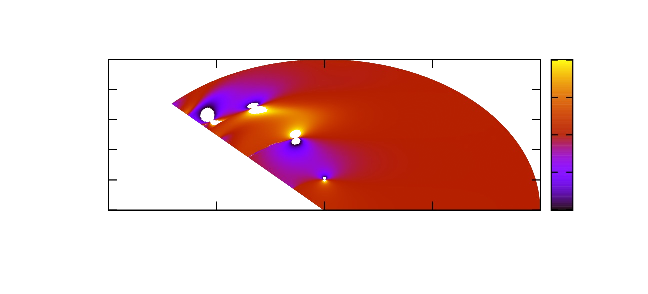
\includegraphics{monopole_anal_f_real}}%
    \gplfronttext
  \end{picture}%
\endgroup

  \end{frame}

  \begin{frame}
    \frametitle{Analytic continuation of the Monopole}
    Real part of the gauge field:
    % GNUPLOT: LaTeX picture with Postscript
\begingroup
  \makeatletter
  \providecommand\color[2][]{%
    \GenericError{(gnuplot) \space\space\space\@spaces}{%
      Package color not loaded in conjunction with
      terminal option `colourtext'%
    }{See the gnuplot documentation for explanation.%
    }{Either use 'blacktext' in gnuplot or load the package
      color.sty in LaTeX.}%
    \renewcommand\color[2][]{}%
  }%
  \providecommand\includegraphics[2][]{%
    \GenericError{(gnuplot) \space\space\space\@spaces}{%
      Package graphicx or graphics not loaded%
    }{See the gnuplot documentation for explanation.%
    }{The gnuplot epslatex terminal needs graphicx.sty or graphics.sty.}%
    \renewcommand\includegraphics[2][]{}%
  }%
  \providecommand\rotatebox[2]{#2}%
  \@ifundefined{ifGPcolor}{%
    \newif\ifGPcolor
    \GPcolortrue
  }{}%
  \@ifundefined{ifGPblacktext}{%
    \newif\ifGPblacktext
    \GPblacktexttrue
  }{}%
  % define a \g@addto@macro without @ in the name:
  \let\gplgaddtomacro\g@addto@macro
  % define empty templates for all commands taking text:
  \gdef\gplbacktext{}%
  \gdef\gplfronttext{}%
  \makeatother
  \ifGPblacktext
    % no textcolor at all
    \def\colorrgb#1{}%
    \def\colorgray#1{}%
  \else
    % gray or color?
    \ifGPcolor
      \def\colorrgb#1{\color[rgb]{#1}}%
      \def\colorgray#1{\color[gray]{#1}}%
      \expandafter\def\csname LTw\endcsname{\color{white}}%
      \expandafter\def\csname LTb\endcsname{\color{black}}%
      \expandafter\def\csname LTa\endcsname{\color{black}}%
      \expandafter\def\csname LT0\endcsname{\color[rgb]{1,0,0}}%
      \expandafter\def\csname LT1\endcsname{\color[rgb]{0,1,0}}%
      \expandafter\def\csname LT2\endcsname{\color[rgb]{0,0,1}}%
      \expandafter\def\csname LT3\endcsname{\color[rgb]{1,0,1}}%
      \expandafter\def\csname LT4\endcsname{\color[rgb]{0,1,1}}%
      \expandafter\def\csname LT5\endcsname{\color[rgb]{1,1,0}}%
      \expandafter\def\csname LT6\endcsname{\color[rgb]{0,0,0}}%
      \expandafter\def\csname LT7\endcsname{\color[rgb]{1,0.3,0}}%
      \expandafter\def\csname LT8\endcsname{\color[rgb]{0.5,0.5,0.5}}%
    \else
      % gray
      \def\colorrgb#1{\color{black}}%
      \def\colorgray#1{\color[gray]{#1}}%
      \expandafter\def\csname LTw\endcsname{\color{white}}%
      \expandafter\def\csname LTb\endcsname{\color{black}}%
      \expandafter\def\csname LTa\endcsname{\color{black}}%
      \expandafter\def\csname LT0\endcsname{\color{black}}%
      \expandafter\def\csname LT1\endcsname{\color{black}}%
      \expandafter\def\csname LT2\endcsname{\color{black}}%
      \expandafter\def\csname LT3\endcsname{\color{black}}%
      \expandafter\def\csname LT4\endcsname{\color{black}}%
      \expandafter\def\csname LT5\endcsname{\color{black}}%
      \expandafter\def\csname LT6\endcsname{\color{black}}%
      \expandafter\def\csname LT7\endcsname{\color{black}}%
      \expandafter\def\csname LT8\endcsname{\color{black}}%
    \fi
  \fi
  \setlength{\unitlength}{0.0500bp}%
  \begin{picture}(6236.00,2834.00)%
    \gplgaddtomacro\gplbacktext{%
    }%
    \gplgaddtomacro\gplfronttext{%
      \csname LTb\endcsname%
      \put(1046,517){\makebox(0,0){\strut{}-10}}%
      \put(2082,517){\makebox(0,0){\strut{}-5}}%
      \put(3118,517){\makebox(0,0){\strut{} 0}}%
      \put(4154,517){\makebox(0,0){\strut{} 5}}%
      \put(5190,517){\makebox(0,0){\strut{} 10}}%
      \put(3118,187){\makebox(0,0){\strut{}$x$}}%
      \put(874,803){\makebox(0,0)[r]{\strut{} 0}}%
      \put(874,1093){\makebox(0,0)[r]{\strut{} 2}}%
      \put(874,1383){\makebox(0,0)[r]{\strut{} 4}}%
      \put(874,1671){\makebox(0,0)[r]{\strut{} 6}}%
      \put(874,1961){\makebox(0,0)[r]{\strut{} 8}}%
      \put(874,2251){\makebox(0,0)[r]{\strut{} 10}}%
      \put(412,1527){\rotatebox{-270}{\makebox(0,0){\strut{}$y$}}}%
      \put(5633,811){\makebox(0,0)[l]{\strut{}-5}}%
      \put(5633,1288){\makebox(0,0)[l]{\strut{} 0}}%
      \put(5633,1764){\makebox(0,0)[l]{\strut{} 5}}%
      \put(5633,2241){\makebox(0,0)[l]{\strut{} 10}}%
    }%
    \gplbacktext
    \put(0,0){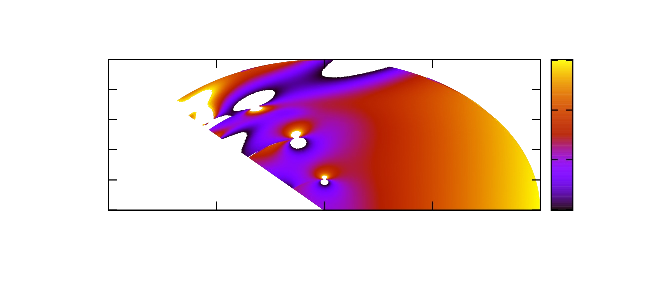
\includegraphics{monopole_anal_h_real}}%
    \gplfronttext
  \end{picture}%
\endgroup

  \end{frame}
\end{section}

\begin{section}{Conclusions \& Future Work}
  \begin{frame}
    \frametitle{Conclusions \& Future Work}
    \begin{itemize}
    \item Numerical framework to find the analytical continuation of a function,
    \item Successfully tested on a set of different situations,
    \item Proved on the numerical level that the Wick rotation of the abelian vortex and non-abelian vortex is valid.
    \item Additional arguments are required in order to corroborate numerical results.
    \end{itemize}
  \end{frame}
  \begin{frame}
    \frametitle{Questions?}
  \end{frame}
\end{section}
